\section{mo\-Simple\-Move\-Tabu\-List$<$ M $>$ Class Template Reference}
\label{classmo_simple_move_tabu_list}\index{moSimpleMoveTabuList@{moSimpleMoveTabuList}}
Class describing a move tabu list with a limited memory.  


{\tt \#include $<$mo\-Simple\-Move\-Tabu\-List.h$>$}

Inheritance diagram for mo\-Simple\-Move\-Tabu\-List$<$ M $>$::\begin{figure}[H]
\begin{center}
\leavevmode
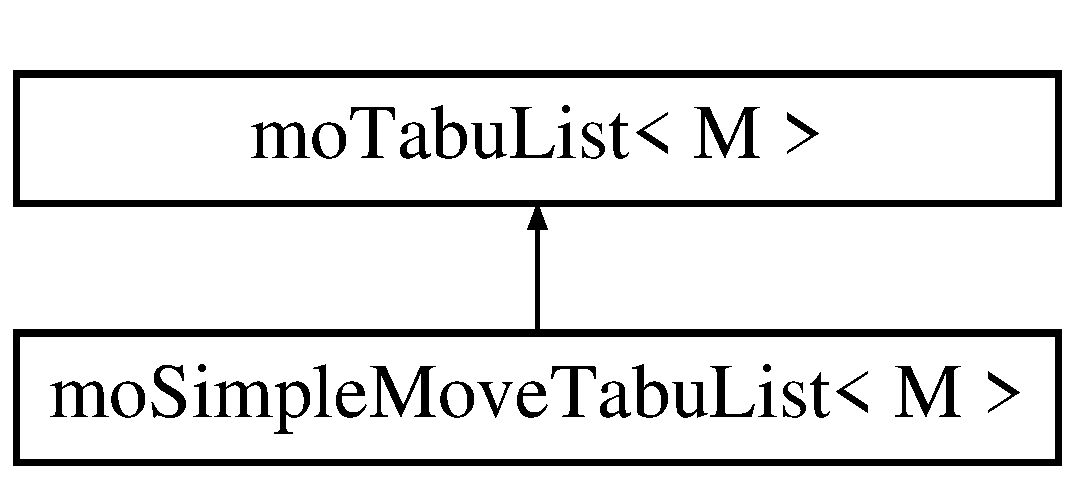
\includegraphics[height=4cm]{classmo_simple_move_tabu_list}
\end{center}
\end{figure}
\subsection*{Public Types}
\begin{CompactItemize}
\item 
typedef M::EOType {\bf EOT}\label{classmo_simple_move_tabu_list_w0}

\begin{CompactList}\small\item\em Alias for the type. \item\end{CompactList}\item 
typedef std::list$<$ M $>$::iterator {\bf move\-Iterator}\label{classmo_simple_move_tabu_list_w1}

\begin{CompactList}\small\item\em Alias for an iterator of a move list. \item\end{CompactList}\end{CompactItemize}
\subsection*{Public Member Functions}
\begin{CompactItemize}
\item 
{\bf mo\-Simple\-Move\-Tabu\-List} (unsigned int \_\-memory\_\-maximum\_\-size)\label{classmo_simple_move_tabu_list_a0}

\begin{CompactList}\small\item\em Constructor. \item\end{CompactList}\item 
bool {\bf operator()} (const M \&\_\-move, const {\bf EOT} \&\_\-solution)
\begin{CompactList}\small\item\em Function that indicates if, in a given state, the \_\-move is tabu or not. \item\end{CompactList}\item 
void {\bf add} (const M \&\_\-move, const {\bf EOT} \&\_\-solution)
\begin{CompactList}\small\item\em Procedure to add a move in the tabu list. \item\end{CompactList}\item 
void {\bf update} ()
\begin{CompactList}\small\item\em Procedure that updates the tabu list content. \item\end{CompactList}\item 
void {\bf init} ()
\begin{CompactList}\small\item\em Procedure which initialises the tabu list. \item\end{CompactList}\end{CompactItemize}
\subsection*{Private Member Functions}
\begin{CompactItemize}
\item 
void {\bf remove\-Move} (const M \&\_\-move)
\begin{CompactList}\small\item\em Procedure that removes a given move from the tabu list (if it is into, else do nothing). \item\end{CompactList}\end{CompactItemize}
\subsection*{Private Attributes}
\begin{CompactItemize}
\item 
unsigned int {\bf memory\_\-maximum\_\-size}\label{classmo_simple_move_tabu_list_r0}

\begin{CompactList}\small\item\em The maximum size of the tabu list. \item\end{CompactList}\item 
unsigned int {\bf memory\_\-size}\label{classmo_simple_move_tabu_list_r1}

\begin{CompactList}\small\item\em The current size of the tabu list. \item\end{CompactList}\item 
std::list$<$ M $>$ {\bf tabu\-List}\label{classmo_simple_move_tabu_list_r2}

\begin{CompactList}\small\item\em The move tabu list. \item\end{CompactList}\end{CompactItemize}


\subsection{Detailed Description}
\subsubsection*{template$<$class M$>$ class mo\-Simple\-Move\-Tabu\-List$<$ M $>$}

Class describing a move tabu list with a limited memory. 



Definition at line 46 of file mo\-Simple\-Move\-Tabu\-List.h.

\subsection{Member Function Documentation}
\index{moSimpleMoveTabuList@{mo\-Simple\-Move\-Tabu\-List}!operator()@{operator()}}
\index{operator()@{operator()}!moSimpleMoveTabuList@{mo\-Simple\-Move\-Tabu\-List}}
\subsubsection{\setlength{\rightskip}{0pt plus 5cm}template$<$class M$>$ bool {\bf mo\-Simple\-Move\-Tabu\-List}$<$ M $>$::operator() (const M \& {\em \_\-move}, const {\bf EOT} \& {\em \_\-solution})\hspace{0.3cm}{\tt  [inline]}}\label{classmo_simple_move_tabu_list_a1}


Function that indicates if, in a given state, the \_\-move is tabu or not. 

\begin{Desc}
\item[Parameters:]
\begin{description}
\item[{\em \_\-move}]A given {\bf mo\-Move}{\rm (p.\,\pageref{classmo_move})}. \item[{\em \_\-solution}]A solution. \end{description}
\end{Desc}
\begin{Desc}
\item[Returns:]true or false. \end{Desc}


Definition at line 69 of file mo\-Simple\-Move\-Tabu\-List.h.

References mo\-Simple\-Move\-Tabu\-List$<$ M $>$::EOT, mo\-Simple\-Move\-Tabu\-List$<$ M $>$::move\-Iterator, and mo\-Simple\-Move\-Tabu\-List$<$ M $>$::tabu\-List.\index{moSimpleMoveTabuList@{mo\-Simple\-Move\-Tabu\-List}!add@{add}}
\index{add@{add}!moSimpleMoveTabuList@{mo\-Simple\-Move\-Tabu\-List}}
\subsubsection{\setlength{\rightskip}{0pt plus 5cm}template$<$class M$>$ void {\bf mo\-Simple\-Move\-Tabu\-List}$<$ M $>$::add (const M \& {\em \_\-move}, const {\bf EOT} \& {\em \_\-solution})\hspace{0.3cm}{\tt  [inline, virtual]}}\label{classmo_simple_move_tabu_list_a2}


Procedure to add a move in the tabu list. 

The two parameters have not to be modified so they are constant parameters.

\begin{Desc}
\item[Parameters:]
\begin{description}
\item[{\em \_\-move}]a new tabu move. \item[{\em \_\-solution}]the origianl solution associated to this move. \end{description}
\end{Desc}


Implements {\bf mo\-Tabu\-List$<$ M $>$} {\rm (p.\,\pageref{classmo_tabu_list_a0})}.

Definition at line 86 of file mo\-Simple\-Move\-Tabu\-List.h.

References mo\-Simple\-Move\-Tabu\-List$<$ M $>$::EOT, mo\-Simple\-Move\-Tabu\-List$<$ M $>$::memory\_\-size, mo\-Simple\-Move\-Tabu\-List$<$ M $>$::remove\-Move(), and mo\-Simple\-Move\-Tabu\-List$<$ M $>$::tabu\-List.\index{moSimpleMoveTabuList@{mo\-Simple\-Move\-Tabu\-List}!update@{update}}
\index{update@{update}!moSimpleMoveTabuList@{mo\-Simple\-Move\-Tabu\-List}}
\subsubsection{\setlength{\rightskip}{0pt plus 5cm}template$<$class M$>$ void {\bf mo\-Simple\-Move\-Tabu\-List}$<$ M $>$::update ()\hspace{0.3cm}{\tt  [inline, virtual]}}\label{classmo_simple_move_tabu_list_a3}


Procedure that updates the tabu list content. 

Generally, a counter associated to each saved move is decreased by one. 

Implements {\bf mo\-Tabu\-List$<$ M $>$} {\rm (p.\,\pageref{classmo_tabu_list_a1})}.

Definition at line 110 of file mo\-Simple\-Move\-Tabu\-List.h.\index{moSimpleMoveTabuList@{mo\-Simple\-Move\-Tabu\-List}!init@{init}}
\index{init@{init}!moSimpleMoveTabuList@{mo\-Simple\-Move\-Tabu\-List}}
\subsubsection{\setlength{\rightskip}{0pt plus 5cm}template$<$class M$>$ void {\bf mo\-Simple\-Move\-Tabu\-List}$<$ M $>$::init ()\hspace{0.3cm}{\tt  [inline, virtual]}}\label{classmo_simple_move_tabu_list_a4}


Procedure which initialises the tabu list. 

Can be useful if the data structure needs to be allocated before being used. 

Implements {\bf mo\-Tabu\-List$<$ M $>$} {\rm (p.\,\pageref{classmo_tabu_list_a2})}.

Definition at line 115 of file mo\-Simple\-Move\-Tabu\-List.h.\index{moSimpleMoveTabuList@{mo\-Simple\-Move\-Tabu\-List}!removeMove@{removeMove}}
\index{removeMove@{removeMove}!moSimpleMoveTabuList@{mo\-Simple\-Move\-Tabu\-List}}
\subsubsection{\setlength{\rightskip}{0pt plus 5cm}template$<$class M$>$ void {\bf mo\-Simple\-Move\-Tabu\-List}$<$ M $>$::remove\-Move (const M \& {\em \_\-move})\hspace{0.3cm}{\tt  [inline, private]}}\label{classmo_simple_move_tabu_list_d0}


Procedure that removes a given move from the tabu list (if it is into, else do nothing). 

\begin{Desc}
\item[Parameters:]
\begin{description}
\item[{\em \_\-move}]A given {\bf mo\-Move}{\rm (p.\,\pageref{classmo_move})}. \end{description}
\end{Desc}


Definition at line 126 of file mo\-Simple\-Move\-Tabu\-List.h.

References mo\-Simple\-Move\-Tabu\-List$<$ M $>$::move\-Iterator, and mo\-Simple\-Move\-Tabu\-List$<$ M $>$::tabu\-List.

Referenced by mo\-Simple\-Move\-Tabu\-List$<$ M $>$::add().

The documentation for this class was generated from the following file:\begin{CompactItemize}
\item 
mo\-Simple\-Move\-Tabu\-List.h\end{CompactItemize}
